\subsection{Esercizio 22}
Tabulare il massimo errore di approssimazione (stimato su 10001 punti equidistanti
in $[0, 1]$) ottenuto approssimando le funzioni
\[
    \begin{array}{ccccc}
        sin(2\pi x) & & e & & cos(2\pi x)
    \end{array}
\]
mediante le function $spline0$ e $spline$, interpolanti su $n + 1$ punti equidistanti in $[0, 1]$,
per $n = 5, 10, 15, 20, \dots, 50$. Commentare i risultati ottenuti.
\newline \textbf{Soluzione:}

Eseguendo lo script \nameref{cod:22} si ottengono i risultati contenuti nella tabella \ref{tab:22}
e nella figura \ref{fig:es22}, che rappresenta il logaritmo di errore di interpolazione data
eccessiva differenza tra alcuni valori.
\begin{table}[h]
    \renewcommand\arraystretch{2}
    \resizebox{\columnwidth}{!}{
        \begin{tabular}{| l l l l l l|}
            \hline
            Numero di punti & \vline & spline0 sin           & spline sin            & spline0 cos           & spline cos            \\
            \hline
            5               & \vline & 2.001701314863913e-02 & 1.807582872673141e-01 & 1.610187576696707e-01 & 2.001701314863924e-02 \\
            10              & \vline & 6.866934777143285e-04 & 4.406993304975182e-03 & 2.548906760377223e-02 & 4.997949001644519e-03 \\
            15              & \vline & 1.110611957051422e-04 & 5.108853724136997e-04 & 1.015096384509251e-02 & 1.022458829215145e-03 \\
            20              & \vline & 3.189430039152175e-05 & 1.128798996133107e-04 & 5.445736215755059e-03 & 3.179572242010265e-04 \\
            25              & \vline & 1.233796729405157e-05 & 3.536684739838258e-05 & 3.394941446614230e-03 & 1.278076383067761e-04 \\
            30              & \vline & 5.797512077632128e-06 & 1.378425643952519e-05 & 2.318648806181711e-03 & 6.067991993707889e-05 \\
            35              & \vline & 3.063198617536678e-06 & 6.237243845463869e-06 & 1.684034317896432e-03 & 3.234496704618284e-05 \\
            40              & \vline & 1.764375267554463e-06 & 3.145724463402000e-06 & 1.278527355775938e-03 & 1.876829765667942e-05 \\
            45              & \vline & 1.085622804652964e-06 & 1.722751742837259e-06 & 1.003721436690030e-03 & 1.162001372967403e-05 \\
            50              & \vline & 7.065852024590313e-07 & 1.006498800408540e-06 & 8.089237478392519e-04 & 7.571318735410948e-06 \\
            \hline
        \end{tabular}
    }
    \caption{valori approssimati con i metodi spline0 e spline}
    \label{tab:22}
\end{table}
\begin{figure}[!ht]
    \centering
    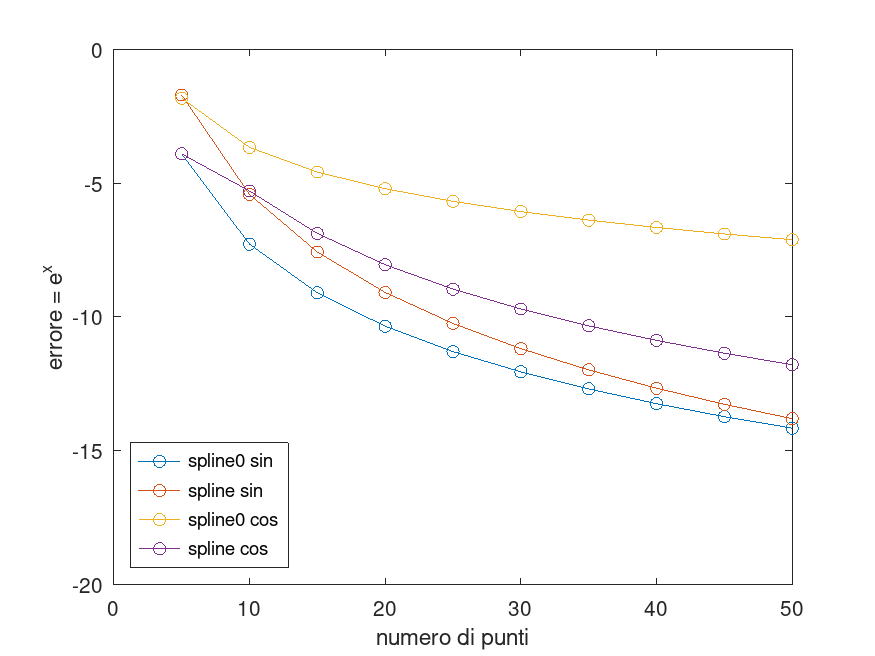
\includegraphics[width=16cm,height=12cm,keepaspectratio]{capitolo5/es22_figure.png}
    \caption{logaritmo di errore}
    \label{fig:es22}
\end{figure}
\FloatBarrier
In base ai risultati ottenuti, si constata che la spline knot-a-not implementata da
Matlab restituisce degli errori di approssimazione significativamente più bassi
per quanto riguarda la funzione $f(x) = cos(2 \pi x)$. Si osserva invece che i risultati
ottenuti per $f(x) = sin(2 \pi x)$ si discostano meno tra di loro. Il motivo di ciò è
che le spline cubiche naturali hanno un piccolo errore agli estremi dovuto alle
condizioni iniziali imposte. Ovvero, data $f(x) = cos(2 \pi x)$:
\[
    f'(0) = f''(1) = -4 \pi ^2
\]
Osserviamo che questo errore non si presenta con $f(x) = sin(2 \pi x)$. Infatti:
\[
    f''(0) = f''(1) = 0
\]
